Deadlock is a critical problem in Network-on-Chip systems, where a group of packets are permanently blocked because each of them is waiting for resources held by others. In packet-switched networks, deadlock usually occurs when packets form a cyclic dependency on channels or buffers, so that none of them can continue to move forward, as shown in Figure~\ref{fig:deadlock}.

\begin{figure}[htbp]
    \centering
    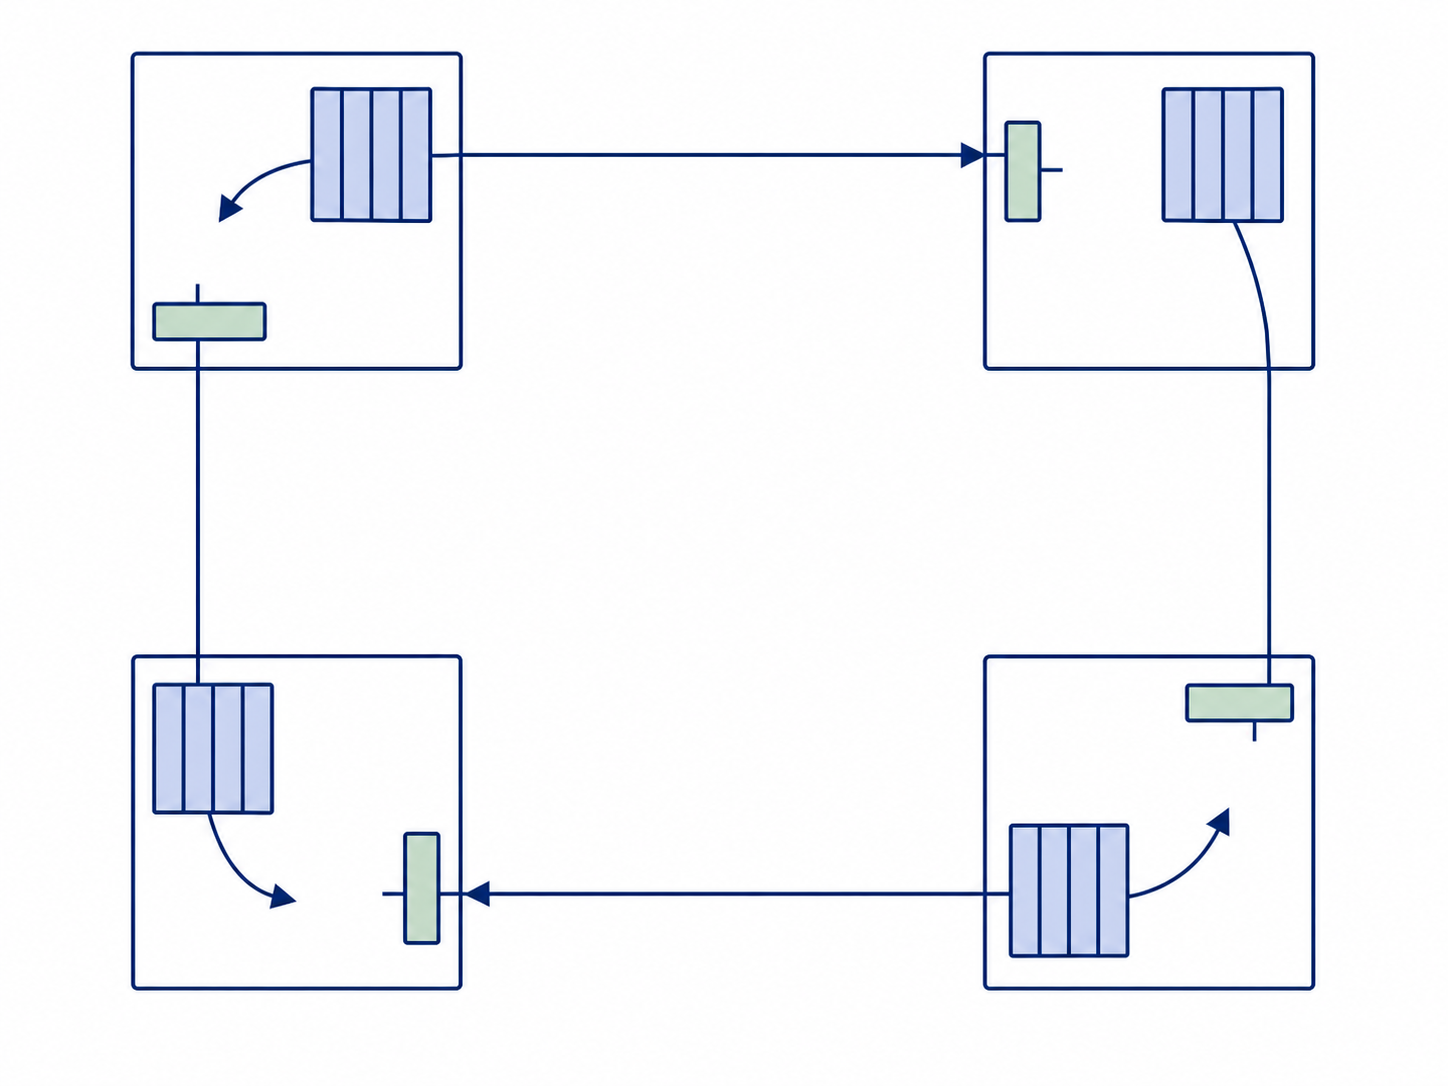
\includegraphics[width=0.6\textwidth]{images/ch2background/deadlock.png}
    \caption{Deadlock scenario caused by cyclic dependency}
    \label{fig:deadlock}
\end{figure}

In wormhole-switched NoCs, deadlock is closely related to buffer occupation and channel allocation. Since packets advance flit by flit and may hold network resources while waiting for the next channel to become available, circular waiting can arise when several packets occupy different resources and simultaneously request one another’s blocked paths. Once such a cycle is formed, the involved packets remain stalled indefinitely unless additional recovery mechanisms are introduced.

Because deadlock can completely stop packet delivery and significantly degrade network reliability, it must be considered carefully in router and routing design. In general, deadlock can be avoided either by designing routing algorithms that eliminate cyclic channel dependencies or by introducing mechanisms such as virtual channels to separate traffic flows and break resource dependency cycles.